%%
%% CalculatorLab (c) 2021 Christopher A. Bohn
%%
%% Licensed under the Apache License, Version 2.0 (the "License");
%% you may not use this file except in compliance with the License.
%% You may obtain a copy of the License at
%%     http://www.apache.org/licenses/LICENSE-2.0
%% Unless required by applicable law or agreed to in writing, software
%% distributed under the License is distributed on an "AS IS" BASIS,
%% WITHOUT WARRANTIES OR CONDITIONS OF ANY KIND, either express or implied.
%% See the License for the specific language governing permissions and
%% limitations under the License.
%%

%%
%% (c) 2021 Christopher A. Bohn
%%

\documentclass[12pt]{article}

\usepackage{fullpage}
\usepackage{fancyhdr}
\usepackage[procnames]{listings}
\usepackage{hyperref}
\usepackage{textcomp}
\usepackage{bold-extra}
\usepackage[dvipsnames]{xcolor}
\usepackage{etoolbox}


% Customize the semester (or quarter) and the course number

\newcommand{\courseterm}{Spring 2022}
\newcommand{\coursenumber}{CSCE 231}

% Customize how a typical lab will be managed;
% you can always use \renewcommand for one-offs

\newcommand{\runtimeenvironment}{your account on the \textit{csce.unl.edu} Linux server}
\newcommand{\filesource}{Canvas or {\footnotesize$\sim$}cse231 on \textit{csce.unl.edu}}
\newcommand{\filesubmission}{Canvas}

% These are placeholder commands and will be renewed in each lab

\newcommand{\labnumber}{}
\newcommand{\labname}{Lab \labnumber\ Assignment}
\newcommand{\shortlabname}{}
\newcommand{\duedate}{}

% Individual or team effort

\newcommand{\individualeffort}{This is an individual-effort project. You may discuss concepts and syntax with other students, but you may discuss solutions only with the professor and the TAs. Sharing code with or copying code from another student or the internet is prohibited.}
\newcommand{\teameffort}{This is a team-effort project. You may discuss concepts and syntax with other students, but you may discuss solutions only with your assigned partner(s), the professor, and the TAs. Sharing code with or copying code from a student who is not on your team, or from the internet, is prohibited.}
\newcommand{\freecollaboration}{In addition to the professor and the TAs, you may freely seek help on this assignment from other students.}
\newcommand{\collaborationrules}{}

% Do you care about software engineering?

\providebool{allowspaghetticode}

\setbool{allowspaghetticode}{false}

\newcommand{\softwareengineeringfrontmatter}{
    \ifboolexpe{not bool{allowspaghetticode}}{
        \section*{No Spaghetti Code Allowed}
        In the interest of keeping your code readable, you may \textit{not} use
        any \lstinline{goto} statements, nor may you use any \lstinline{break}
        statements to exit from a loop, nor may you have any functions
        \lstinline{return} from within a loop.
    }{}
}

\newcommand{\spaghetticodepenalties}[1]{
    \ifboolexpe{not bool{allowspaghetticode}}{
        \penaltyitem{1}{for each \lstinline{goto} statement, \lstinline{break}
            statement used to exit from a loop, or \lstinline{return} statement
            that occurs within a loop.}
    }{}
}

% You shouldn't need to customize these,
% but you can if you like

\lstset{language=C, tabsize=4, upquote=true, basicstyle=\ttfamily}
\newcommand{\function}[1]{\textbf{\lstinline{#1}}}
\setlength{\headsep}{0.7cm}
\hypersetup{colorlinks=true}

\newcommand{\startdocument}{
    \pagestyle{fancy}
    \fancyhf{}
    \lhead{\coursenumber}
    \chead{\ Lab \labnumber: \labname}
    \rhead{\courseterm}
    \cfoot{\shortlabname-\thepage}

	\begin{document}
	\title{\ Lab \labnumber}
	\author{\labname}
	\date{Due: \duedate}
	\maketitle

    \textit{\collaborationrules}
}

\newcommand{\rubricitem}[2]{\item[\underline{\hspace{1cm}} +#1] #2}
\newcommand{\bonusitem}[2]{\item[\underline{\hspace{1cm}} Bonus +#1] #2}
\newcommand{\penaltyitem}[2]{\item[\underline{\hspace{1cm}} -#1] #2}

%%
%% labs/common/semester.tex
%% (c) 2021-22 Christopher A. Bohn
%%
%% Licensed under the Apache License, Version 2.0 (the "License");
%% you may not use this file except in compliance with the License.
%% You may obtain a copy of the License at
%%     http://www.apache.org/licenses/LICENSE-2.0
%% Unless required by applicable law or agreed to in writing, software
%% distributed under the License is distributed on an "AS IS" BASIS,
%% WITHOUT WARRANTIES OR CONDITIONS OF ANY KIND, either express or implied.
%% See the License for the specific language governing permissions and
%% limitations under the License.
%%


% Customize the semester (or quarter) and the course number

\newcommand{\courseterm}{Fall 2022}
\newcommand{\coursenumber}{CSCE 231}

% Customize how a typical lab will be managed;
% you can always use \renewcommand for one-offs

\newcommand{\runtimeenvironment}{your account on the \textit{csce.unl.edu} Linux server}
\newcommand{\filesource}{Canvas or {\footnotesize$\sim$}cse231 on \textit{csce.unl.edu}}
\newcommand{\filesubmission}{Canvas}

% Customize for the I/O lab hardware

\newcommand{\developmentboard}{Arduino Nano}
%\newcommand{\serialprotocol}{SPI}
\newcommand{\serialprotocol}{I2C}
%\newcommand{\displaymodule}{MAX7219digits}
%\newcommand{\displaymodule}{MAX7219matrix}
\newcommand{\displaymodule}{LCD1602}

\setbool{usedisplayfont}{true}

\newcommand{\obtaininghardware}{
    The EE Shop has prepared ``class kits'' for CSCE 231; your class kit costs \$30.
    The EE Shop is located at 122 Scott Engineering Center and is open M-F 7am-4pm. You do not need an appointment.
    You may pay at the window with cash, with a personal check, or with your NCard.
    The EE shop does \textit{not} accept credit cards.
}

% Update to reflect the CS2 course(s) at your institute

\newcommand{\cstwo}{CSCE~156, RAIK~184H, or SOFT~161}

% Do you care about software engineering?

\setbool{allowspaghetticode}{false}

% Which assignments are you using this semester, and when are they due?

\newcommand{\pokerlabnumber}{1}
\newcommand{\pokerlabcollaboration}{
    Sections~\ref{sec:connecting}, \ref{sec:terminology}, \ref{sec:gettingstarted}, \ref{subsec:typesofpokerhands}, and~\ref{subsec:studythecode}: \freecollaboration
    Sections~\ref{sec:completingcard} and~\ref{subsec:completepoker}: \individualeffort
}
\newcommand{\pokerlabdue}{Week of August 29, before the start of your lab section}

\newcommand{\keyboardlabnumber}{2}
\newcommand{\keyboardlabcollaboration}{\individualeffort}
\newcommand{\keyboardlabdue}{Week of January 31, before the start of your lab section}

\newcommand{\pointerlabnumber}{3}
\newcommand{\pointerlabcollaboration}{\individualeffort}
\newcommand{\pointerlabdue}{Week of February 7, before the start of your lab section}

\newcommand{\integerlabnumber}{4}
\newcommand{\integerlabcollaboration}{\individualeffort}
\newcommand{\integerlabdue}{Week of February 14, before the start of your lab section}

\newcommand{\floatlabnumber}{5}
\newcommand{\floatlabcollaboration}{\individualeffort}
\newcommand{\floatlabdue}{soon}

\newcommand{\addressinglabnumber}{6}
\newcommand{\addressinglabcollaboration}{\individualeffort}
\newcommand{\addressinglabdue}{Week of February 28, before the start of your lab section}

%bomblab was 7
%attacklab was 8

\newcommand{\pollinglabnumber}{9}
\newcommand{\pollinglabcollaboration}{\individualeffort}
\newcommand{\pollinglabdue}{Week of April 11, before the start of your lab section}
\newcommand{\pollinglabenvironment}{your \developmentboard-based class hardware kit}

\newcommand{\ioprelabnumber}{\pollinglabnumber-prelab}
\newcommand{\ioprelabcollaboration}{\freecollaboration}
\newcommand{\ioprelabdue}{Before the start of your lab section on April 5 or 6}

\newcommand{\interruptlabnumber}{10}
\newcommand{\interruptlabcollaboration}{\individualeffort}
\newcommand{\interruptlabdue}{Week of April 18, before the start of your lab section}
\newcommand{\interruptlabenvironment}{your \developmentboard-based class hardware kit}

\newcommand{\capstonelab}{ComboLock}    % this will come into play when we generalize capstonelab
\newcommand{\capstonelabnumber}{11}
\newcommand{\capstonelabcollaboration}{\teameffort}
\newcommand{\capstonelabdue}{Week of May 2, Before the start of your lab section\footnote{See Piazza for the due dates of teams with students from different lab sections.}}
\newcommand{\capstonelabenvironment}{your \developmentboard-based class hardware kit}

\newcommand{\memorylabnumber}{12}
\newcommand{\memorylabcollaboration}{This is an individual-effort project. You may discuss the nature of memory technologies and of memory hierarchies with classmates, but you must draw your own conclusions.}
\newcommand{\memorylabdue}{Week of May 2, at the end of your lab section}
\newcommand{\memorylabenvironment}{your \developmentboard-based class hardware kit and your account on the \textit{csce.unl.edu} Linux server}

% Labs not used this semester

\newcommand{\concurrencylabnumber}{XX}
\newcommand{\concurrencylabcollaboration}{\individualeffort}
\newcommand{\concurrencylabdue}{not this semester}

\newcommand{\ssbcwarmupnumber}{XX}
\newcommand{\ssbcwarmupcollaboration}{\freecollaboration}
\newcommand{\ssbcwarmupdue}{not this semester}

\newcommand{\ssbcpollingnumber}{XX}
\newcommand{\ssbcpollingcollaboration}{\individualeffort}
\newcommand{\ssbcpollingdue}{not this semester}

\newcommand{\ssbcinterruptnumber}{XX}
\newcommand{\ssbcinterruptcollaboration}{\individualeffort}
\newcommand{\ssbcinterruptdue}{not this semester}

\usepackage{graphicx}
%\usepackage{media9}
\usepackage{addfont}
\addfont{OT1}{d7seg}{\dviiseg}
% \addfont{OT1}{deseg}{\deseg}
%\usepackage[normalem]{ulem}
%\usepackage{subfig}
\usepackage{wrapfig}
%\usepackage{animate}
% \usepackage{multicol}
\usepackage{enumitem}

\renewcommand{\labnumber}{\capstonelabnumber}
\renewcommand{\labname}{Using Interrupt-Driven Input/Output}
\renewcommand{\shortlabname}{interrupt-driven i/o -- calculatorlab}
\renewcommand{\collaborationrules}{\capstonelabcollaboration}
\renewcommand{\duedate}{\capstonelabdue}
\newcommand{\nano}{\developmentboard} % TODO: replace \nano with \developmentboard
\renewcommand{\runtimeenvironment}{\capstonelabenvironment}
\pagelayout
\begin{document}
\labidentifier

In this assignment, you will write code for \runtimeenvironment\ that will use
interrupts from external devices and from a timer to drive some of the logic
for a four-function calculator.

\begin{figure}[h]
    \centering
    
\includegraphics[width=10cm]{MomMomMom}
    \caption{Interrupts. \tiny Image by 20th Century Fox Television}
\end{figure}

The instructions are written assuming you will edit the code in the Arduino IDE
and run it on \runtimeenvironment, constructed according to the pre-lab
instructions. If you wish, you may edit the code in a different environment;
however, our ability to provide support for problems with other IDEs is limited.

Please familiarize yourself with the entire assignment before beginning.
Section~\ref{sec:FunctionalSpecification} has the functional specification of
the system you will develop -- the integer calculator specification is
required; the fractional calculator specification is extra-credit.
Section~\ref{sec:Constraints} describes implementation constraints.
Section~\ref{sec:TimerInterrupts} guides you in creating and handling timer
interrupts using the AVR-libc \function{ISR()} macro, and
Section~\ref{sec:ExternalInterrupts} guides you in handling external interrupts
using the Arduino core \function{attachInterrupt()} function. Finally,
Section~\ref{sec:Calculator} has a few thoughts on implementing the calculator
functionality.

\section{Four-Function Calculator Specification} \label{sec:FunctionalSpecification}

\subsection*{Integer Calculator}

\begin{enumerate}
\item \label{spec:IntegerCalculator} The calculator shall be an
    infix\footnote{\url{https://en.wikipedia.org/wiki/Calculator_input_methods\#Infix_notation}}
    decimal calculator capable of performing addition, subtraction,
    multiplication, and division.
    \begin{itemize}
    \item If only integer behavior is implemented, then division shall be
        integer division; \textit{i.e.}, the fractional portion of quotients
        values shall be truncated.
    \end{itemize}
\item \label{spec:NoDecimalPoint} A decimal point shall not be displayed.
\item Each arithmetic operation shall use two operands, referred in this
    specification as \textit{operand1} and \textit{operand2}.
    \begin{itemize}
    \item Because no further history of operands is maintained, the algebraic
        order of operations is not preserved.
    \item The value of \textit{operand1} can only be changed as the result of a
        calculation or by clearing its value.
    \item The value of \textit{operand2} is ``built'' through keypresses on the
        matrix keypad.
    \item \textit{operand1} and \textit{operand2} are defined in the problem
        domain. Your solution space might not have direct corollaries (for
        example, in the problem domain, \textit{operand2} can be undefined,
        which is not a characteristic of any number types in C).
    \end{itemize}
\item The \textbf{7-segment display module} shall display \textit{operand1}'s
    value except when building \textit{operand2}, except when an error
    condition is present, and except when the display is disabled.
\item Initially, \textit{operand1} shall hold the value 0, \textit{operand2}
    shall have no defined value, and no arithmetic operation shall be specified.
\item \label{spec:BuildingValue} When building \textit{operand2}:
    \begin{enumerate}
    \item When the user starts to build \textit{operand2}, \textit{operand1}
        shall no longer be displayed. Instead, the value being built shall be
        displayed.
    \item Except as otherwise specified in requirement~\ref{spec:Wakening},
        whenever the user presses a numeral button on the \textbf{matrix
        keypad}, the corresponding digit shall be displayed in the
        least-significant position of the \textbf{7-segment display module},
        and any digits already displayed shall increase in significance by one
        order of magnitude. For example, if {\dviiseg 234} is displayed and the
        user presses \texttt{5} then {\dviiseg 2345} shall be displayed.
    \item Except as otherwise specified in requirement~\ref{spec:Wakening},
        whenever the user presses the \textbf{left pushbutton}, the value being
        displayed shall be negated.
        \begin{itemize}
        \item If \textit{operand2} has a defined value (is being built) then
            \textit{operand2} shall be negated.
        \item If \textit{operand2} has no defined value (\textit{operand1} is
            displayed) then \textit{operand1} shall be negated.
        \end{itemize}
    \item In no case shall the calculator allow the user to input a value
        requiring more digits than can be displayed on the \textbf{7-segment
        display module}. If the user attempts to enter a value that requires
        more digits, then the value shall remain unchanged.
    \end{enumerate}
\item \label{spec:Negative} If a negative value is displayed, the negative sign
    shall be displayed immediately to the left of the most-significant digit
    being displayed. For example, {\dviiseg-456} is correctly displayed, but
    {\dviiseg -    456} is not correctly displayed.
\item \label{spec:Positive} A positive sign shall not be displayed as part of a
    positive decimal value.
\item \label{spec:LeadingZeroes} Leading 0s shall not be displayed. For
    example, {\dviiseg 782} is correctly displayed, but {\dviiseg 00000782} is
    not correctly displayed. However, when the value to be displayed is 0, then
    {\dviiseg 0} shall be displayed.
\item The \texttt{A} button indicates addition. The \texttt{B} button indicates
    subtraction. The \texttt{C} button indicates multiplication. The \texttt{D}
    button indicates division. The \texttt{\#} button directs that the
    calculation shall be executed without specifying another arithmetic
    operation.
\item Except as otherwise specified in requirement~\ref{spec:Wakening}, when
    the user presses the \texttt{\#} button, directing that the calculation is
    to be executed, the \underline{previously}-specified operation shall be
    performed, the resulting value shall become \textit{operand1} (and shall be
    displayed), and there shall no longer be a valid \textit{operand2}. If
    there was no previously-specified operation, then \textit{operand2} shall
    become \textit{operand1}, and there shall no longer be a valid
    \textit{operand2}.
\item Except as otherwise specified in requirement~\ref{spec:Wakening}, when
    the user presses an operation button (\texttt{A}-\texttt{D}), the
    \underline{previously}-specified operation shall be performed, the
    resulting value shall become \textit{operand1} (and shall be displayed),
    there shall no longer be a valid \textit{operand2}, and the next operation
    to be performed shall be that which corresponds to the button pressed. If
    there was no previously-specified operation, then \textit{operand2} shall
    become \textit{operand1}, \textit{operand2} shall no longer have a defined
    value, and the \underline{next} operation to be performed shall be that
    which corresponds to the button pressed.
    \begin{itemize}
    \item If the resulting value (\textit{operand1}) is too great to be
        displayed, the \textbf{7-segment display module} shall display
        {\dviiseg Error}.
    \item If \textit{operand2} is 0 and the operation is division, the
        \textbf{7-segment display module} shall display {\dviiseg Error}.
    \end{itemize}
\item The calculator shall not support scientific notation, neither for operand
    entry nor for displaying a result.
\item Except as otherwise specified in requirement~\ref{spec:Wakening},
    whenever the user presses the \textbf{right pushbutton}:
    \begin{enumerate}
    \item If \textit{operand2} is being built, then \textit{operand2} shall be
        reset to no defined value, the next operation (if any) shall be
        cleared, and \textit{operand1} shall be displayed.
    \item If \textit{operand2} is not being built, then \textit{operand1} shall
        be reset to 0 (and 0 shall be displayed), and the next operation (if
        any) shall be cleared.
    \end{enumerate}
\item Display timeout: If no button or key has been pressed for a designated
    amount of time, the \textbf{7-segment display module} shall go blank;
    however, \textit{operand1}, \textit{operand2} being built (if any), and the
    next operation (if any) shall be retained. When the \textbf{left switch} is
    in the left position, the designated time is \underline{exactly 30
    seconds}; when the \textbf{left switch} is in the right position, the
    designated time is \underline{exactly 5 seconds}.
    \begin{itemize}
    \item Do not place the microcontroller in Idle mode, nor any other Sleep
        mode.
    \end{itemize}
\item \label{spec:Wakening} If the display has timed out, then pressing any key
    or button will cause the display to resume displaying its previous output.
    The key/button press that takes the display out of its timed-out mode shall
    not otherwise affect the system's state; specifically, it shall not
    contribute to \textit{operand2}'s value, it shall not cause an operation to
    be executed, it shall not specify an operation to be performed, nor shall
    it clear any operands or specified operations.
\end{enumerate}

Figure~\ref{fig:StateDiagram} depicts a problem-space state diagram of the
4-function integer calculator, not including too-great values, and not
including display's time-out and resume-display behavior.

\begin{figure}
    \centering
    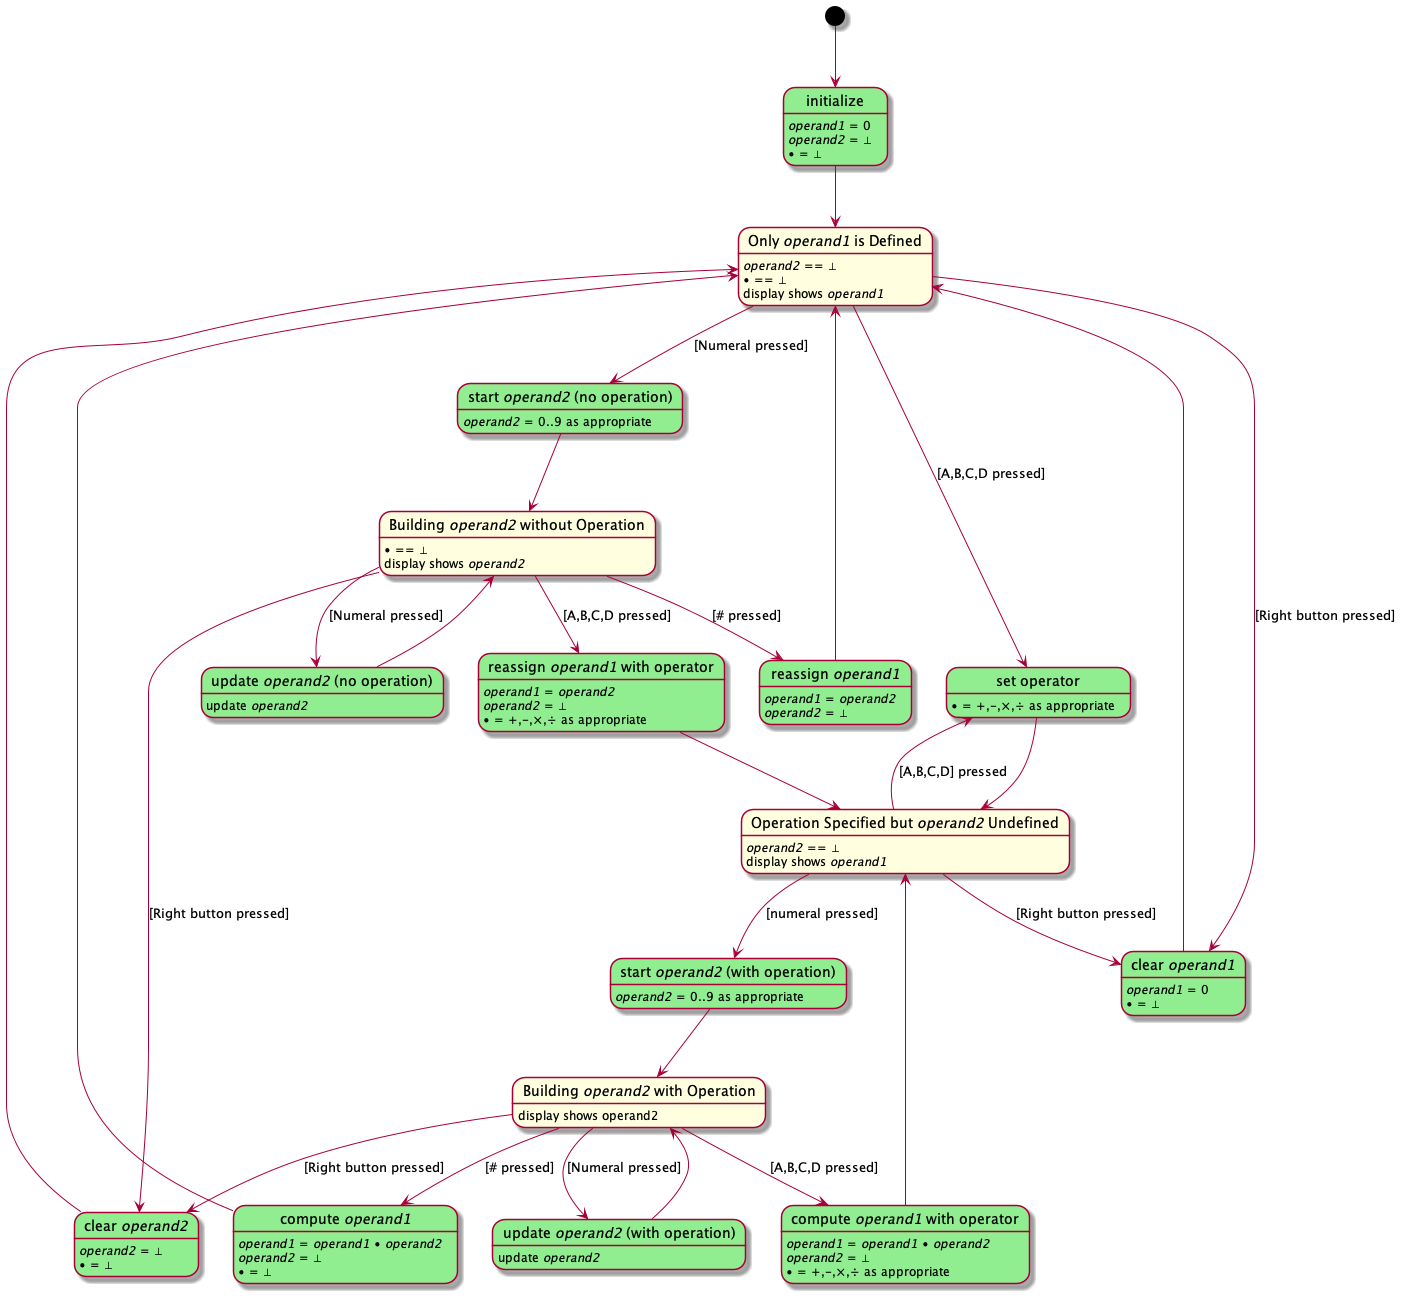
\includegraphics[width=18cm]{CalculatorStateDiagram}
    \caption{\label{fig:StateDiagram} State diagram depicting ``normal''
        behavior for integer calculator. Yellow states depict invariant
        conditions; green states depict updates to the problem-domain variables
        \textit{operand1}, \textit{operand2}, and $\bullet$ (operator). \tiny
        Diagram by Bohn}
\end{figure}

\subsection*{Fractional Calculator}

If fractional-value behavior is implemented, then the calculator's
specification is amended and extended:

\begin{enumerate}[resume]
\item Requirement~\ref{spec:NoDecimalPoint} is replaced with: \\
    A decimal point shall be displayed as necessary:
    \begin{enumerate}
    \item The decimal point, when displayed, shall not occupy a full display
        position in the \textbf{7-segment display module}; instead, it shall be
        occupy the \texttt{DP} segment of the same display position as the
        ones-place digit.
    \item When \textit{operand1} is displayed, it shall always include a
        decimal point.
    \item When \textit{operand2} is displayed, the decimal point shall not be
        displayed unless the \texttt{*} button has been pressed (see
        requirement~\ref{spec:DecimalPointButton}).
    \item If the value being displayed is an integer value and a decimal point
        is required, then the decimal point shall be displayed after the
        least-significant digit (for example: {\dviiseg 123.}). If the value
        being displayed has a fractional portion, then the decimal point shall
        be displayed between the ones-place and the tenths-place (for example,
        $123\frac{1}{4}$ shall be displayed as {\dviiseg 123.25}).
    \end{enumerate}
\item The clarification sub-bullet for requirement~\ref{spec:IntegerCalculator}
    is replaced with: \\
    Division shall be conventional division; \textit{i.e.}, the fractional
    portion of quotients, if any, shall be displayed in accordance with the
    rounding rule of requirement~\ref{spec:Rounding}.
\item Requirement~\ref{spec:LeadingZeroes} is amended: If the value to be
    displayed is between -1.0 and 1.0, exclusive, then a {\dviiseg 0} shall be
    displayed in the ones-place.
\item Trailing 0s in the fractional portion of a value shall not be displayed.
    For example, {\dviiseg 231.8} is correctly displayed, but {\dviiseg
    231.80000} is not correctly displayed.
\item \label{spec:DecimalPointButton} The \texttt{*} key can be thought of
    as the decimal point key; that is, any keys pressed before pressing the
    \texttt{*} key shall be part of the integer portion of the value being
    built, and any keys pressed after pressing the \texttt{*} key shall be
    part of the fractional portion of the value being built.
\item \label{spec:Rounding} If the total number of digits required to display
    the integer portion and the fractional portion of \textit{operand1}
    (including the negative sign if needed) exceeds the number of digits in the
    \textbf{7-segment display module}) then the value shall be rounded:
    \begin{enumerate}
    \item All display positions shall be used.
    \item If the most-significant digit of the truncated portion is less than
        5, then the value shall be rounded toward zero (\textit{i.e.}, the
        least-significant displayed digit shall be unchanged). For example,
        12345.6782 shall be displayed as {\dviiseg 12345.678} after rounding.
    \item If the most-significant digit of the truncated portion is greater
        than 5, or if that digit is 5 and there are more digits that follow,
        then the value shall be rounded away from zero. For example, both
        12345.6789 and 12345.67851 shall be displayed as {\dviiseg 12345.679}
        after rounding.
    \item If the most-significant digit of the truncated portion is 5 and there
        are no digits that follow (``exactly halfway'') then the value shall be
        rounded in whichever direction makes the least-significant displayed
        digit even (0, 2, 4, 6, or 8). For example, both 12345.6775 and
        12345.6785 shall be displayed as {\dviiseg 12345.678} after rounding.
    \end{enumerate}
    \begin{itemize}
    \item If the value is too small to be displayed (the value is between
        -0.0000005 and 0.00000005, inclusive, which round to 0) then {\dviiseg
        0} shall be displayed. A negative value that rounds to 0 shall not
        preserve its negative sign.
    \item If the value is too great to be displayed after rounding (the
        resulting integer portion requires more digits than are available) then
        the value shall not be rounded; instead, {\dviiseg Error} shall be
        displayed.
    \end{itemize}
\end{enumerate}

\section{Constraints}\label{sec:Constraints}

You may continue to use the memory-mapped I/O registers, or you can use
functions provided by the Arduino core read from and write to pins.

You may re-use code from the previous lab, or you can rewrite the necessary
code using functions, macros, types, or constants that are part of the Arduino
core;\footnote{\url{https://www.arduino.cc/reference/en/}} functions, macros,
types, or constants of
avr-libc;\footnote{\url{https://www.nongnu.org/avr-libc/user-manual/index.html}}
or one of Arduino's standard
libraries.\footnote{\url{https://www.arduino.cc/reference/en/libraries/} The
standard libraries are those under the heading, ``Standard Libraries.''} You
may \textit{not} use a third-party library, not even one that the Arduino
Libraries reference page links to (if it isn't among those available in the
Arudino IDE's ``Sketch'' $\rightarrow$ ``Include Library'' menu under
``Arduino libraries'' then you may not use it).

You may \textit{not} poll the matrix keypad nor the pushbuttons to determine
if they have been pressed. You must use interrupts to determine if a key or
button has been pressed. Once a press has been detected, you may scan the
matrix keypad or read the pushbuttons to determine which key or button has
been pressed.

While it is possible to configure the SPI hardware to generate an interrupt
after the content of the SPI Data Register is transmitted, you may use your
\function{send_data()} function that polls the \texttt{SPIF} bit.

You may poll the left switch to determine if its position has changed;
however, the specification has been written such that your code should only
need to occasionally check the switch's position rather than polling it for
changes.

While you may use \function{millis()} for debouncing, you may \textit{not} use
\function{millis()} nor \function{micros()} to implement the display timeout.
You must use an interrupt from the ATmega328's Timer1 or Timer2 as part of
implementing the display timeout.

\section{Getting Started} \label{sec:GettingStarted}

Open the Arduino IDE. Create a new sketch by selecting from the menu ``File''
$\rightarrow$ ``New''. Select ``File'' $\rightarrow$ ``Save As\dots'' and save
it as \textit{CalculatorLab}. Using File Explorer (Windows), Finder (MacOS), an
equivalent file manager (Linux), or a command-line terminal, copy
\textit{cowpi.h} from your \texttt{Arduino/PollingLab} directory into your
\texttt{Arduino/CalculatorLab} directory. In the Arduino IDE, add
\lstinline{#include "cowpi.h"} to the top of \textit{CalculatorLab.ino}.

Optionally copy the following code from your \textit{PollingLab.ino} into your
\textit{CalculatorLab.ino}:
    \begin{itemize}
    \item \lstinline{struct gpio_registers *gpio},
        \lstinline{struct spi_registers *spi},
        \lstinline{const uint8_t keys[][]}, and
        \lstinline{const uint8_t seven_segments[]}
    \item \function{setup()} (replacing the \function{setup()} function in
        \textit{CalculatorLab.ino}), \function{setup_simple_io()},
        \function{setup_keypad()}, and \function{setup_display_module()}
    \item \function{get_key_pressed()} and \function{display_data()}
    \end{itemize}

If you need to rewrite any of the code from the previous lab, you may do so
without explicitly using the memory-mapped I/O registers. You may instead use
\function{pinMode()}\footnote{\url{https://www.arduino.cc/reference/en/language/functions/digital-io/pinmode/}}$^\mathrm{,}$\footnote{\url{https://www.arduino.cc/en/Tutorial/Foundations/DigitalPins}}
to configure the pins, and \function{digitalRead()}\footnote{\url{https://www.arduino.cc/reference/en/language/functions/digital-io/digitalread/}}
and \function{digitalWrite()}\footnote{\url{https://www.arduino.cc/reference/en/language/functions/digital-io/digitalwrite/}}
to perform input and output on specific pins. You may use the Arduino SPI
library\footnote{\url{https://www.arduino.cc/en/Reference/SPI}} to use the
ATmega328's SPI hardware to send data to the display module, but you will
probably find it easier to use \function{shiftOut()}\footnote{\url{https://www.arduino.cc/reference/en/language/functions/advanced-io/shiftout/}}
(see \function{SendData()} in the prelab's \textit{DisplayTest.ino} for an
example).

You may want to keep your code from the PollingLab's ``conversion mode'' handy,
but don't copy it into \textit{CalculatorLab.ino} since it uses polling to
detect the user pressing keys and buttons.

\section{Implementing Timeout}\label{sec:TimerInterrupts}

You must use timer interrupts from either Timer1 or Timer2 as part of your
implementation of the display timeout. Without using an external clock source,
you won't be able to configure an interrupt to occur every 30 seconds, or even
every 5 seconds. Since we will not use an external clock source, you will need
to use timer interrupts along with other logic.

\subsection{Preparation}

Design your logic and determine how often you need a timer interrupt to make it
work. For example, the \nano's pseudorealtime clock relies on an interrupt from
Timer0 every 1.024µs and advances the millisecond counter after 1,000 of these
interrupts have occurred. The pseudorealtime clock uses an overflow-based timer
interrupt to arrive at an approximation of milliseconds. The calculator's
specification calls for the display module going black exactly 5 seconds or
exactly 30 seconds (depending on the switch position) after the last key press
or button press. To achieve exactness, you will use a comparison-based timer.

You can then determine the parameters for the timer using
this equation:
\[
16,000,000 \frac{\mathrm{cycles}}{\mathrm{second}} =
    comparison\_value \frac{\mathrm{beats}}{\mathrm{interrupt}} \times
    prescaler \frac{\mathrm{cycles}}{\mathrm{beat}} \times
    interrupt\_frequency \frac{\mathrm{interrupts}}{\mathrm{second}}
\]
or, equivalently:
\[
    comparison\_value \frac{\mathrm{beats}}{\mathrm{interrupt}} \times
    prescaler \frac{\mathrm{cycles}}{\mathrm{beat}} =
    16,000,000 \frac{\mathrm{cycles}}{\mathrm{second}} \times
    interrupt\_period \frac{\mathrm{seconds}}{\mathrm{interrupt}}
\]
where:
    \begin{description}
    \item [16,000,000 Hz] is the clock frequency (the inverse of the clock
        period).
    \item [comparison\_value] is a number you will place in one of the
        timer's \texttt{compare} registers for a comparison-based timer
        interrupt. This can be any possible value of an unsigned 16-bit integer
        for Timer1, or any possible value of an unsigned 8-bit integer for
        Timer2.
    \item [prescaler] is a multiplier applied to the clock period to adjust the
        time between counter increments (``beats''). Possible values are 1, 8,
        64, 256, and 1024 for Timer1, or 1, 8, 32, 64, 128, 256, and 1024 for
        Timer2.
    \item [interrupt\_frequency] is how often you want a timer interrupt (the
        inverse of the interrupt period).
    \item [interrupt\_period] is the time between timer interrupts (the
        inverse of the interrupt frequency).
    \end{description}

You may have to iterate on your design until you arrive at one that works with
the constraints of that equation's terms for whichever timer you choose to use.

The Waveform Generation Mode you will use is \textit{CTC} (Clear Timer on
Compare) with the ``TOP'' value set by the \texttt{OCRnA} (\textit{compareA})
register, where $n$ is the Timer number. Use Figure~\ref{fig:Timer1WGM} (for
Timer1) or Figure~\ref{fig:Timer2WGM} (for Timer2) to select the appropriate
\texttt{WGM13}~\texttt{WGM12}~\texttt{WGM11}~\texttt{WGM10} or
\texttt{WGM22}~\texttt{WGM21}~\texttt{WGM20} bits.

Based on the prescaler you chose for the above equation, select the appropriate
\texttt{CS12}~\texttt{CS11}~\texttt{CS10} or
\texttt{CS22}~\texttt{CS20}~\texttt{CS20} bits from Figure~\ref{fig:Timer1CS}
(for Timer1) or Figure~\ref{fig:Timer2CS}) (for Timer2).

\subsection{Setup}

In the \function{setup()} function or a function called by \function{setup()}:

You may configure the timer using either memory-mapped I/O or using macros
provided by AVR-libc.\footnote{AVR-libc provides macros named after the I/O
registers that allow you to read from and write to these registers as though
they were ordinary variables.} If using memory-mapped I/O:
\begin{itemize}
\item For Timer1, create a pointer to a
    \lstinline{struct timer_registers_16bit} and assign to it the address
    \lstinline{IObase + 0x60}.
\item For Timer2, create a pointer to a
    \lstinline{struct timer_registers_8bit} and assign to it the address
    \lstinline{IObase + 0x90}.
\item Use the struct's \lstinline{control} field to set the \texttt{WGM} and
    \texttt{CS} bits in the timer's control registers.
    \begin{itemize}
    \item Use Tables~\ref{table:Timer1Registers} and \ref{table:Timer1Control}
        (for Timer1) or Tables~\ref{table:Timer2Registers} and
        \ref{table:Timer2Control} (for Timer2) to determine where the
        \texttt{WGM} and \texttt{CS} bits are located in the control registers.
    \end{itemize}
\end{itemize}

If using AVR-libc macros:
\begin{itemize}
\item For Timer1, make assignments to \lstinline{TCCR1A} and/or
    \lstinline{TCCR1B}.
\item For Timer2, make assignments to \lstinline{TCCR2A} and/or
    \lstinline{TCCR2B}.
\item Use Table~\ref{table:Timer1Control} (for Timer1)
    Table~\ref{table:Timer2Control} (for Timer2) to determine where the
    \texttt{WGM} and \texttt{CS} bits are located in the control registers.
\end{itemize}

\begin{figure}
    \centering
    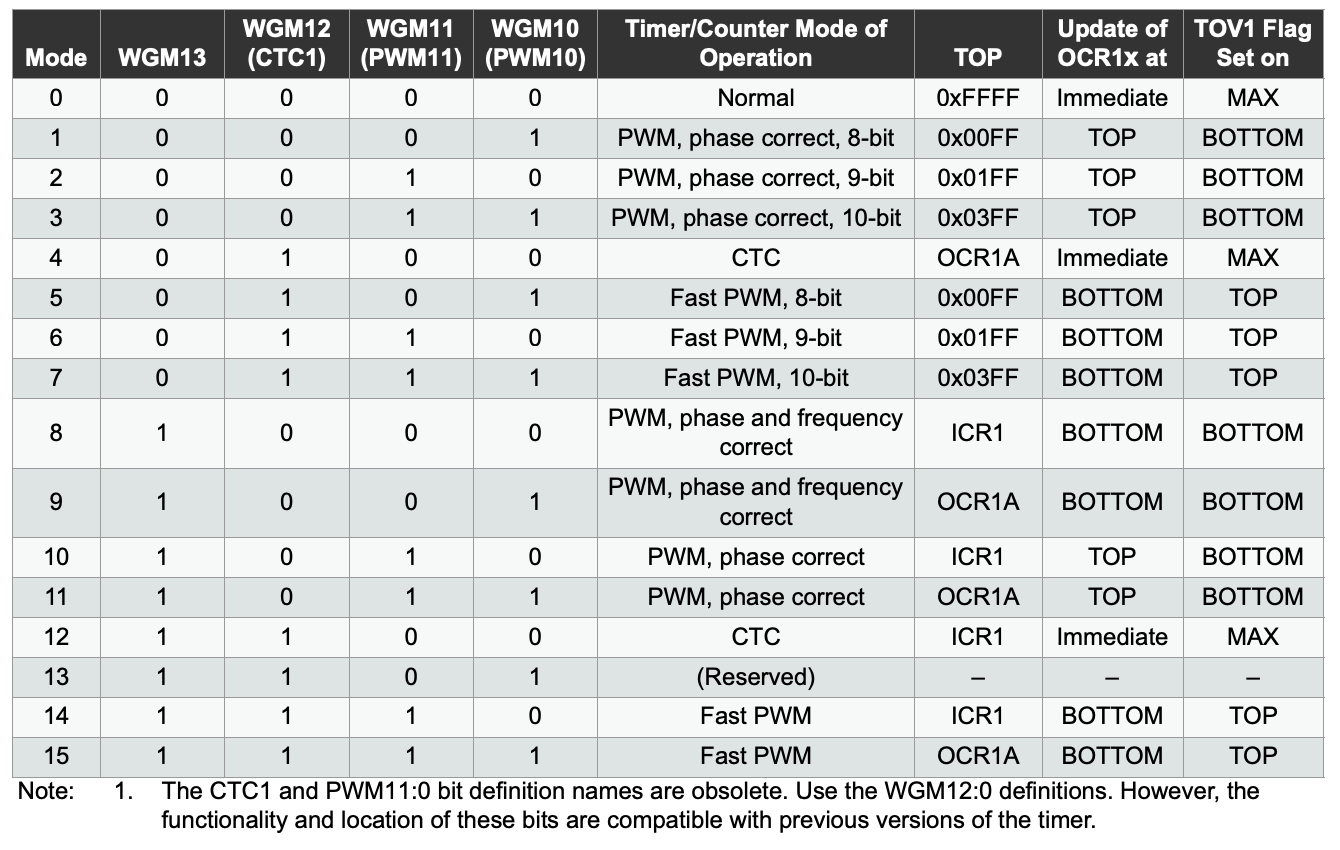
\includegraphics[width=15cm]{WGM-Timer1}
    \caption{Waveform Generation Mode Bit Description for Timer1. \tiny Copied from ATmega382P Data Sheet, Table~15-5 \label{fig:Timer1WGM}}
\end{figure}

\begin{figure}
    \centering
    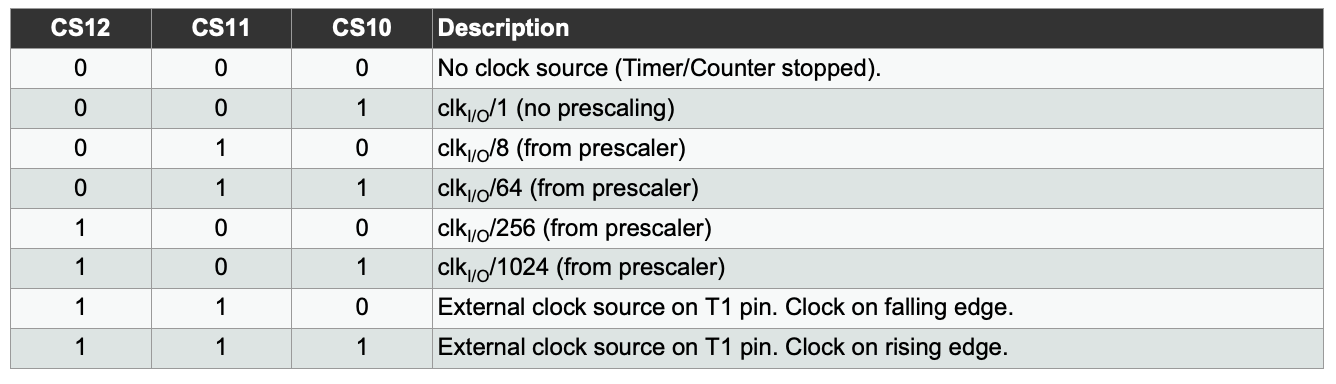
\includegraphics[width=15cm]{CS-Timer1}
    \caption{Clock Select Bit Description for Timer1. \tiny Copied from ATmega382P Data Sheet, Table~15-6 \label{fig:Timer1CS}}
\end{figure}

\begin{figure}
    \centering
    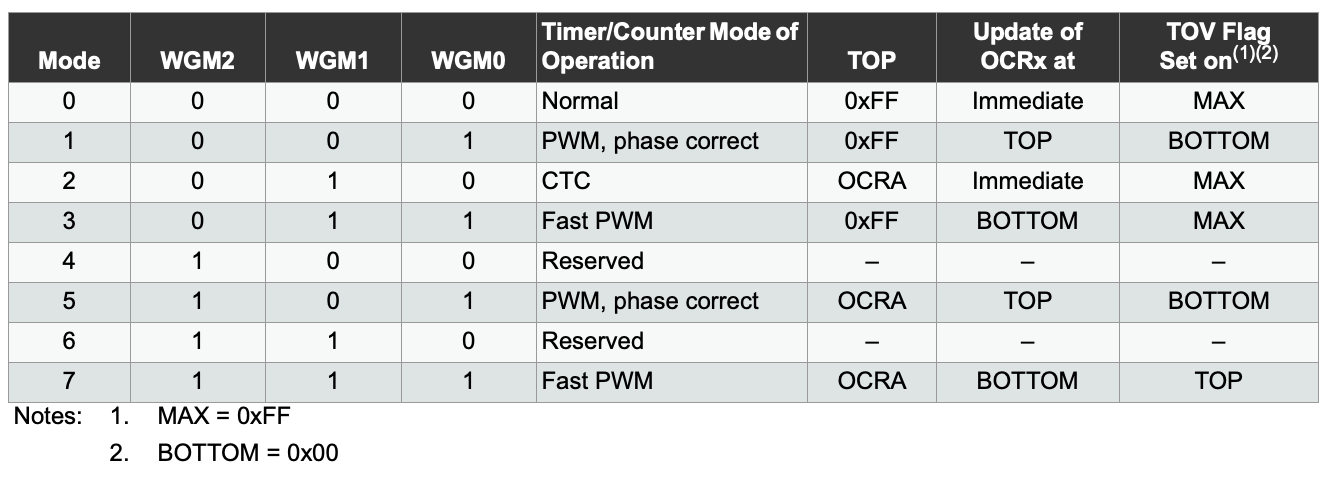
\includegraphics[width=15cm]{WGM-Timer2}
    \caption{Waveform Generation Mode Bit Description for Timer2. \texttt{WGM22}, \texttt{WGM21}, and \texttt{WGM20} are incorrectly shown here as \texttt{WGM2}, \texttt{WGM1}, and \texttt{WGM0}. \texttt{OCR2A} is incorrectly shown here as \texttt{OCRA}. \tiny Copied from ATmega382P Data Sheet, Table~17-8 \label{fig:Timer2WGM}}
\end{figure}

\begin{figure}
    \centering
    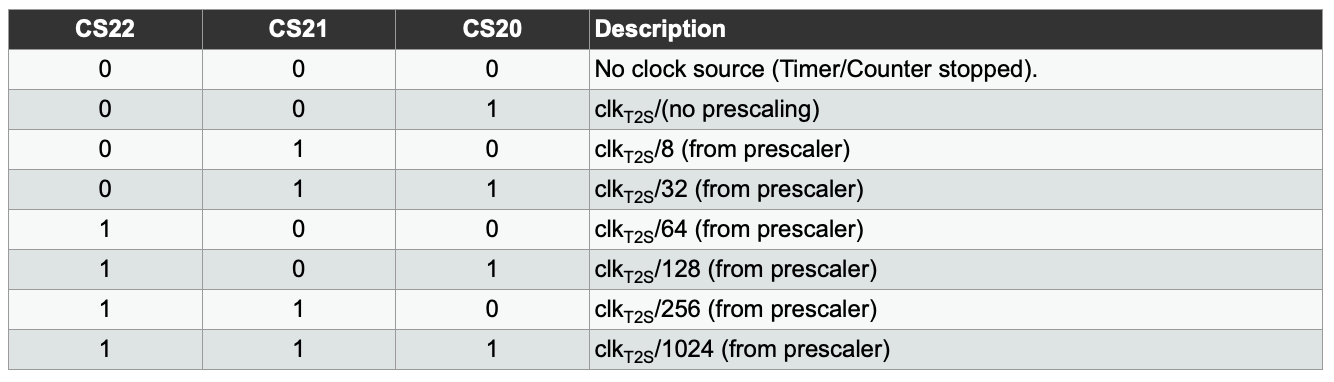
\includegraphics[width=15cm]{CS-Timer2}
    \caption{Clock Select Bit Description for Timer2. \tiny Copied from ATmega382P Data Sheet, Table~17-9 \label{fig:Timer2CS}}
\end{figure}

\begin{table}
    \centering \small
    \begin{tabular}{|r||c|c|c|c||}
        \hline
        Bits                & \textbf{31..24}   & \textbf{23..16}   & \textbf{15..8}    & \textbf{7..0}     \\ \cline{2-5}
        \textbf{control}    & \textit{reserved} & \texttt{TCCR1C}   & \texttt{TCCR1B}   & \texttt{TCCR1A}   \\
        \textbf{counter}    & \multicolumn{2}{c|}{}                 & \multicolumn{2}{c||}{\texttt{TCNT1}}  \\
        \textbf{capture}    & \multicolumn{2}{c|}{}                 & \multicolumn{2}{c||}{\texttt{ICR1}}   \\
        \textbf{compareA}   & \multicolumn{2}{c|}{}                 & \multicolumn{2}{c||}{\texttt{OCR1A}}  \\
        \textbf{compareB}   & \multicolumn{2}{c|}{}                 & \multicolumn{2}{c||}{\texttt{OCR1B}}  \\ \hline
    \end{tabular}
    \caption{Relationship of \lstinline{timer_registers_16bit} fields to Timer1's registers. \tiny Adapted from ATmega382P Data Sheet, §15.11. \label{table:Timer1Registers}}
\end{table}

\begin{table}
    \centering \small
    \begin{tabular}{|r||c|c|c|c|c|c|c|c||}
        \hline
        Bit             & \textbf{7}        & \textbf{6}        & \textbf{5}        & \textbf{4}        & \textbf{3}        & \textbf{2}    & \textbf{1}        & \textbf{0}        \\ \cline{2-9}
        \textbf{TCCR1C} & \texttt{FOC1A}    & \texttt{FOC1B}    & -                 & -                 & -                 & -             & -                 & -                 \\
        \textbf{TCCR1B} & \texttt{ICNC1}    & \texttt{ICES1}    & -                 & \texttt{WGM13}    & \texttt{WGM12}    & \texttt{CS12} & \texttt{CS11}     & \texttt{CS10}     \\
        \textbf{TCCR1A} & \texttt{COM1A1}   & \texttt{COM1A0}   & \texttt{COM1BA1}  & \texttt{COM1B0}   & -                 & -             & \texttt{WGM11}    & \texttt{WGM10}    \\ \hline
    \end{tabular}
    \caption{Timer1's control registers. \tiny Adapted from ATmega382P Data Sheet, §15.11. \label{table:Timer1Control}}
\end{table}

\begin{table}
    \centering \small
    \begin{tabular}{|r||c|c||}
        \hline
        Bits                & \textbf{15..8}    & \textbf{7..0}     \\ \cline{2-3}
        \textbf{control}    & \texttt{TCCR2B}   & \texttt{TCCR2A}   \\
        \textbf{counter}    &                   & \texttt{TCNT2}    \\
        \textbf{compareA}   &                   & \texttt{OCR2A}    \\
        \textbf{compareB}   &                   & \texttt{OCR2B}    \\ \hline
    \end{tabular}
    \caption{Relationship of \lstinline{timer_registers_8bit} fields to Timer2's registers. \tiny Adapted from ATmega382P Data Sheet, §17.11. \label{table:Timer2Registers}}
\end{table}

\begin{table}
    \centering \small
    \begin{tabular}{|r||c|c|c|c|c|c|c|c||}
        \hline
        Bit             & \textbf{7}        & \textbf{6}        & \textbf{5}        & \textbf{4}        & \textbf{3}        & \textbf{2}    & \textbf{1}        & \textbf{0}        \\ \cline{2-9}
        \textbf{TCCR2B} & \texttt{FOC2A}    & \texttt{FOC2B}    & -                 & -                 & \texttt{WGM22}    & \texttt{CS22} & \texttt{CS21}     & \texttt{CS20}     \\
        \textbf{TCCR2A} & \texttt{COM2A1}   & \texttt{COM2A0}   & \texttt{COM2BA1}  & \texttt{COM2B0}   & -                 & -             & \texttt{WGM21}    & \texttt{WGM20}    \\ \hline
    \end{tabular}
    \caption{Timer2's control registers. \tiny Adapted from ATmega382P Data Sheet, §17.11. \label{table:Timer2Control}}
\end{table}

Next assign your computed $comparison\_value$ the struct's \lstinline{compareA}
field, or to OCR1A (Timer1) or OCR2A (Timer2), as appropriate.

Finally, enable the comparison-based timer interrupt. If you are using
memory-mapped I/O:
\begin{itemize}
\item Create a pointer to a \lstinline{volatile uint8_t} and assign to it the
    address \lstinline{IObase + 0x4E}.
\item Treat the pointer as an array, and use the timer number (1 or 2) for the
    index when making an assignment.
\end{itemize}
If you are using AVR-libc macros:
\begin{itemize}
\item Make an assignment to \texttt{TIMSK1} for Timer1, or to \texttt{TIMSK2}
    for Timer2.
\end{itemize}

You want to place a 1 in the \texttt{OCIEnA} bit (where $n$ is the timer
number); use Figure~\ref{fig:TimerInterruptRegisters} to determine the
appropriate bit to set.

\begin{figure}
    \centering
    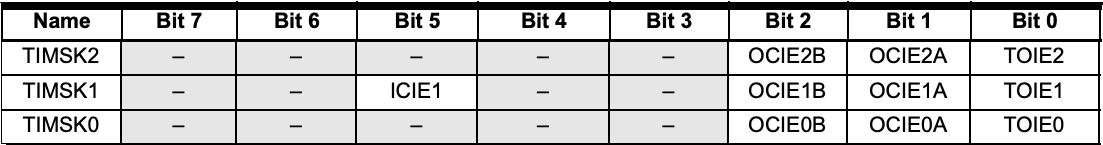
\includegraphics[width=15cm]{TimerInterruptRegisters}
    \caption{Timer interrupt registers. \tiny Cropped from ATmega382P Data Sheet, §30 \label{fig:TimerInterruptRegisters}}
\end{figure}


\subsection{Interrupt Service Routine}

Because the Arduino core does not provide a more convenient way to create an
interrupt service routine (ISR) for timer interrupts, you will use AVR-libc's
\function{ISR}\footnote{\url{https://www.nongnu.org/avr-libc/user-manual/group__avr__interrupts.html}}
macro.

In \textit{CalculatorLab.ino}, outside of any other function, write this code that looks like a function:

\begin{lstlisting}
ISR(vector) {
    ...
}
\end{lstlisting}

where $vector$ is \lstinline{TIMER1_COMPA_vect} for Timer1 or
\lstinline{TIMER2_COMPA_vect} for Timer2. Replace ``\dots'' with the code that
should execute whenever the timer interrupt occurs. You want to keep your ISR
short, no more than a few lines of code. If anything more elaborate needs to
happen, code in your \function{loop()} function (or a function called by
\function{loop()}) can do that based on changes made from within your ISR.

Initially, you may want to simply place a \function{println} statement in your
ISR code to verify that you have the timing correct. Once you are satisfied
that you have done so, remove the \function{println} statement and add the code
you need for your logic.

\textbf{NOTE} Any global variables used by your ISR should be declared as \lstinline{volatile}.

\textbf{NOTE} If you ever need to ``reset'' a timer's count back to 0, you can
simply write 0 to the structs \lstinline{counter} field or to
\texttt{TCNT1}/\texttt{TCNT2}.

\section{Detecting Key and Button Presses}\label{sec:ExternalInterrupts}

For external interrupts, the Arduino core has abstracted-away all of the
configuration details.\footnote{\url{https://www.arduino.cc/reference/en/language/functions/external-interrupts/attachinterrupt/}}
Placing a call to
\begin{lstlisting}
attachInterrupt(digitalPinToInterrupt(pin_number), isr_name, mode);
\end{lstlisting}
will configure all of the necessary registers to call the function
\function{isr_name()} whenever the input value on the pin \textit{pin\_number}
satisfies the \textit{mode}.

\subsection{Setup}

In the \function{setup()} function or a function called by \function{setup()},
configure pins \texttt{D2} and \texttt{D3} for \textbf{high-impedance input}.

Decide on the names of the function that will be called in response to a
keypress on the matrix keypad and of the function that will be called in
response to a button press. For the sake of discussion, I will call these
functions, \function{handle_keypress()} and \function{handle_buttonpress()}.

Recall that the NAND output for the matrix keypad columns provides input to
\texttt{D3} and that the NAND output for the pushbuttons provides input to
\texttt{D2}. Decide on the \textit{mode} for the external interrupts:
    \begin{description}
    \item [LOW] to trigger the interrupt whenever the pin is low
    \item [RISING] to trigger the interrupt whenever the pin goes from low to
        high
    \item [FALLING] to trigger the interrupt whenever the pin goes from high to
        low
    \item [CHANGE] to trigger the interrupt whenever the pin rises or falls
    \end{description}
Because we did not provide a hardware solution to switch bounce, you can expect
both the pin input to both rise and fall a few times when a button or key is
pressed and again when it is released -- but there is no guarantee that
bouncing will occur. For this reason we recommend:
    \begin{itemize}
    \item Use the \lstinline{CHANGE} mode, combined with software debouncing,
        and use a variable to keep track of whether a key or button has been
        pressed (toggle this variable whenever an interrupt occurs, and take
        action based on whether a key or button has been pressed or released).
    \item The software debouncing will look similar to what you used in
        PollingLab except that it only needs to be a few milliseconds instead
        of 500. Since we are not polling the buttons and keypad to detect
        presses, we do not need to worry about the button or key being held for
        several dozen milliseconds being interpretted as multiple presses.
        \begin{itemize}
        \item I very strongly advise against using \function{delay()} for
            software debouncing:
        \item As described in the PollingLab assignment sheet,
            \function{delay()} will leave your system unresponsive to anything
            except interrupts.
        \item Including \function{delay()} calls in an interrupt handler is
            particularly ill-advised since you may find yourself in a situation
            in which you need to disable interrupts in the interrupt handler
            and then re-enable interrupts before exiting the interrupt handler.
            (I do not expect this to happen in this assignment, but I've been
            wrong before.) The \function{delay()} function will never exit,
            blocking forever, if interrupts are disabled.
        \end{itemize}
    \end{itemize}
If you arrive at a different solution that works, you may use your solution.

In the \function{setup()} function or a function called by \function{setup()},
register your ISR functions for the external interrupts:
\begin{lstlisting}
attachInterrupt(digitalPinToInterrupt(2), handle_buttonpress, CHANGE);
attachInterrupt(digitalPinToInterrupt(3), handle_keypress, CHANGE);
\end{lstlisting}
(Here I assumed you would use the CHANGE mode. If you use a different mode,
replace CHANGE with the mode you chose. Similarly, replace
\function{handle_keypress} and \function{handle_buttonpress} with the function
names you chose.)

\subsection{Handling Button Presses}

Your pushbutton handler (``\function{void handle_buttonpress()}'') needs to
determine which button was pressed -- this can be as simple as calling
\lstinline{digitalRead(8)} and \lstinline{digitalRead(9)}. Don't forget to
include software debouncing. If insufficient time (a few milliseconds) has
passed since the last time the button handler was invoked, you can simply exit
the handler function under the assumption that switch bounce is generating
erroneous interrupts.

You might test out your setup with \lstinline{println} statements, but once you
are satisfied with your setup, delete the \lstinline{println} statements and
introduce the code that will actually handle the keypresses.

You want to keep your interrupt handler short. Any time-consuming computations
should happen in your \function{loop()} function (or a function called by
\function{loop()}). If necessary, set global variable(s) value(s) that code in
other functions can use to perform the time-consuming computations. (Reminder:
division, including modulo, is implemented in software on the \nano, and
requires a few-hundred clock cycles to complete.)

Don't forget to reset the 5-second / 30-second countdown so that your code
doesn't blank the display too soon.

Any global variables used by your interrupt handler should be declared as
\lstinline{volatile}.

\subsection{Handling Key Presses}

Your keypad handler (``\function{void handle_keypress()}'') needs to
determine which key was pressed -- you can reuse your
\function{get_key_pressed()} code from PollingLab with minimal changes. One
such change is replacing the code that makes sure the polling treats a keypress
that lasts less than 500ms as a single keypress with code that performs
software debouncing and possible keeping track of whether a CHANGE interrupt is
the result of a key press or a key release. If insufficient time (a few
milliseconds) has passed since the last time the keypad handler was invoked,
you can simply exit the handler function under the assumption that switch
bounce is generating erroneous interrupts.

You might test out your setup with \lstinline{println} statements, but once you
are satisfied with your setup, delete the \lstinline{println} statements and
introduce the code that will actually handle the keypresses.

You want to keep your interrupt handler short. Any time-consuming computations
should happen in your \function{loop()} function (or a function called by
\function{loop()}). If necessary, set global variable(s) value(s) that code in
other functions can use to perform the time-consuming computations. (Reminder:
division, including modulo, is implemented in software on the \nano, and
requires a few-hundred clock cycles to complete.) Almost certainly, you will
want to set a global variable to indicate which key was pressed and then let
\function{loop()} take action based on which key was pressed.

Don't forget to reset the 5-second / 30-second countdown so that your code
doesn't blank the display too soon.

Any global variables used by your interrupt handler should be declared as
\lstinline{volatile}.

\section{Implementing the Calculator}\label{sec:Calculator}

You now have the ability to handle inputs using interrupts. Writing to the
display module can be accomplished with the \function{display_data()} function
you wrote in PollingLab. The logic for ``building'' operands is very similar to
some code you wrote for PollingLab's conversion mode.

The basic Integer Calculator specification is reasonably straight-forward, and
I trust that, given the ability to get input and to display output, any student
who met the course prerequisites can implement it. There are a few nuances that
you will need to address, such as blanking the display and resuming its
display, but I'm confident that you can do that.

The Fractional Calculator, which is extra-credit, is a little more interesting.
You might try using \lstinline{float}s, but you will still need to put a little
effort into displaying the values in accordance with the specification.
Alternatively, you might try the fixed point notation ``hack'' used for decimal
currency that I described earlier in the semester. This would allow you to use
integer types but would need to manually keep track of the decimal point.
Either way, don't forget rounding!


\section*{Turn-in and Grading}

When you have completed this assignment, upload \textit{CalculatorLab.ino} to
\filesubmission.

This assignment is worth 50 points. \\

Rubric:
\begin{description}
\rubricitem{9}{Timer interrupts configured such that, when combined with other
    logic, the software is able to determine when exactly 5 seconds or exactly
    30 seconds has passed since the last key press or button press.}
\rubricitem{1}{Timer ISR is not excessively long.}
\rubricitem{9}{Pushbutton presses are detected with an external interrupt, and
    the handler, at a minimum, determines which button was pressed.}
\rubricitem{1}{Pushbutton interrupt handler is not excessively long.}
\rubricitem{9}{Matrix keypad presses are detected with an external interrupt,
    and the handler, at a minimum, determines which button was pressed.}
\rubricitem{1}{Keypad interrupt handler is not excessively long.}
\rubricitem{1}{Operand is built in accordance with
    requirements~\ref{spec:BuildingValue}, \ref{spec:Negative},
    \ref{spec:Positive}, and \ref{spec:LeadingZeroes}.}
\rubricitem{1}{After eight digits (or a negative sign and seven digits),
    subsequent numeral presses are ignored (except for resetting the
    display-blanking countdown).}
\rubricitem{2}{Addition performs correctly.}
\rubricitem{2}{Subtraction performs correctly.}
\rubricitem{2}{Multiplication performs correctly.}
\rubricitem{2}{Division performs correctly.}
\rubricitem{1}{The result of the previous arithmetic operation can be used as
    the first operand for the next arithmentic operation.}
\rubricitem{1}{Too-great results cause {\dviiseg Error} to be displayed.}
\rubricitem{1}{The ``clear'' button clears the operand being built and any
    specified operation.}
\rubricitem{1}{If no operand is currently being built (the previous
    arithmetic's result is displayed) then the ``clear'' button clears the
    previous arithemtic's result and any specified operation.}
\rubricitem{2}{The display goes blank after exactly 5 seconds or exactly 30
    seconds of inactivity, depending on the position of the left switch.}
\rubricitem{2}{When the display is blank, pressing any button or key causes the
    display to resume\dots}
\rubricitem{2}{\dots and has no other effect, allowing operation to resume where the user had left off before letting the display timeout.}
\bonusitem{5}{Fractional calculator is implemented.}
\bonusitem{2}{Get assignment checked-off by TA or professor during office hours before it is due.}% (Cannot get both bonuses.)}
%\bonusitem{1}{Get assignment checked-off by TA at \textit{start} of your scheduled lab immediately after it is due. (Cannot get both bonuses.)}
\end{description}

\section*{Lab Checkoff}

You are not required to have your assignment checked-off by a TA or the
professor. If you do not do so, then we will perform a functional check
ourselves. In the interest of making grading go faster, we are offering a small
bonus %to get your assignment checked-off at the start of your scheduled lab
% time immediately after it is due. Because checking off all students during lab
% would take up most of the lab time, we are offering a slightly larger bonus
if you complete your assignment early and get it checked-off by a TA or the
professor during office hours.

\textit{Ideally, all team members are present for the check-off; however, only
one team member is necessary for the check-off.}

\begin{enumerate}
\item (\ \ \ ) Establish that the code you are demonstrating is the code you
    submitted to to \filesubmission.
    \begin{itemize}
    % \item If you are getting checked-off during lab time, show the TA that the
    %     file was submitted before it was due.
    \item Download the file into your PollingLab directory. If necessary,
        rename it to \textit{CalculatorLab.ino}.
    \end{itemize}
\item (\ \ \ ) Upload \textit{CalculatorLab.ino} to your \nano.
\item (\ \ \ ) If \textbf{Integer Calculator} then the display shows: \\
    {\dviiseg \phantom{8888888}0} \\
    If \textbf{Fractional Calculator} then the display shows: \\
        {\dviiseg \phantom{8888888}0.} \\
    \textit{Make a note of which calculator was implemented.}
\item (\ \ \ ) Place the left switch in the right position.
\item (\ \ \ ) Enter 123,456; the display shows: \\
    {\dviiseg \phantom{88}123456}
\item (\ \ \ ) \textbf{If you implemented display timeout:} Wait exactly five
    seconds. The display goes blank.
\item (\ \ \ ) \textbf{If you implemented display timeout:} Press 7. The display
    resumes, showing what it previously showed: \\
    {\dviiseg \phantom{88}123456}
\item (\ \ \ ) Press 7. The display shows: \\
    {\dviiseg \phantom{8}1234567}
\item (\ \ \ ) Press \texttt{A} (addition). The display still shows: \\
    {\dviiseg \phantom{8}1234567}
\item (\ \ \ ) Enter 890. The display shows: \\
    {\dviiseg \phantom{88888}890}
\item (\ \ \ ) Press \texttt{\#}. The display shows: \\
    {\dviiseg \phantom{8}1235457} \hspace{1cm} \textit{or} \hspace{1cm}
    {\dviiseg \phantom{8}1235457.}
\item (\ \ \ ) Press the right pushbutton (clear). The display shows: \\
    {\dviiseg \phantom{8888888}0} \hspace{1cm} \textit{or} \hspace{1cm}
    {\dviiseg \phantom{8888888}0.}
\item (\ \ \ ) Place the left switch in the left position.
\item (\ \ \ ) Enter -1,234,567, using the left pushbutton for the negative
    sign. The display shows: \\
    {\dviiseg -1235457}
\item (\ \ \ ) Press 8. The display still shows: \\
    {\dviiseg -1235457}
\item (\ \ \ ) Press \texttt{\#}. The display (still) shows: \\
    {\dviiseg -1235457} \hspace{1cm} \textit{or} \hspace{1cm}
    {\dviiseg -1234567.}
\item (\ \ \ ) Enter 231. The display shows: \\
    {\dviiseg \phantom{88888}231}
\item (\ \ \ ) Press \texttt{B} (subtraction) and enter 321. The display shows: \\
    {\dviiseg \phantom{88888}321}
\item (\ \ \ ) Press \texttt{\#}. The display shows: \\
    {\dviiseg \phantom{88888}-90} \hspace{1cm} \textit{or} \hspace{1cm}
    {\dviiseg \phantom{88888}-90.}
\item (\ \ \ ) Press the right pushbutton (clear). The display shows: \\
    {\dviiseg \phantom{8888888}0} \hspace{1cm} \textit{or} \hspace{1cm}
    {\dviiseg \phantom{8888888}0.}
\item (\ \ \ ) Press \texttt{C} (multiplication) and enter 12. The display
    shows:\\
    {\dviiseg \phantom{888888}12}
\item (\ \ \ ) Press \texttt{\#}. The display shows:\\
    {\dviiseg \phantom{8888888}0} \hspace{1cm} \textit{or} \hspace{1cm}
    {\dviiseg \phantom{8888888}0.}
\item (\ \ \ ) Enter 42. The display shows:\\
    {\dviiseg \phantom{888888}42}
\item (\ \ \ ) Press \texttt{D} (division) and enter 6. The display
    shows:\\
    {\dviiseg \phantom{8888888}6}
\item (\ \ \ ) Press \texttt{\#}. The display shows:\\
    {\dviiseg \phantom{8888888}7} \hspace{1cm} \textit{or} \hspace{1cm}
    {\dviiseg \phantom{8888888}7.}
\item (\ \ \ ) Press \texttt{C} (multiplication) and enter 73. The display
    shows:\\
    {\dviiseg \phantom{888888}73}
\item (\ \ \ ) Press \texttt{\#}. The display shows:\\
    {\dviiseg \phantom{88888}511} \hspace{1cm} \textit{or} \hspace{1cm}
    {\dviiseg \phantom{88888}511.}
\item (\ \ \ ) Press \texttt{C} (multiplication) and enter 200. The display
    shows:\\
    {\dviiseg \phantom{88888}200}
\item (\ \ \ ) Press the right pushbutton (clear). The display shows: \\
    {\dviiseg \phantom{88888}511} \hspace{1cm} \textit{or} \hspace{1cm}
    {\dviiseg \phantom{88888}511.}
\item (\ \ \ ) Press \texttt{C} (multiplication) and enter 200,000. The display
    shows:\\
    {\dviiseg \phantom{88}200000}
\item (\ \ \ ) Press \texttt{\#}. The display shows:\\
    {\dviiseg \phantom{88}Error}
\item (\ \ \ ) \textbf{If you implemented display timeout:}
    \begin{description}
    \item [[ ]] Show the code in which you configured Timer1 or Timer2
    \item [[ ]] Explain the calculation that you used to arrive at your
        comparison value
        \[comparison\_value = 16,000,000 \times interrupt\_period \div prescaler\]
    \item [[ ]] Show and explain the Timer ISR
    \item [[ ]] Show and explain any other code used to implement the display
        timeou
    \item [[ ]] Show and explain the Timer ISR.
    \item [] \textit{If it is not clear to the TA how the display-timeout code
        works, then the TA will:}
    \item [[ ]] Prepare a stopwatch or another timepiece with a ``seconds''
        display (or a ``seconds'' hand)
    \item [[ ]] If necessary, re-activate the display by pressing a button or
        key
    \item [[ ]] Press a button or key on the system at the exact same time as
        starting the stopwatch (or at the exact moment that the ``seconds''
        display/hand hits \textit{00})
    \item [[ ]] Note whether the display clears at exactly 30 seconds and not
        at 30.7 seconds, 29.7 seconds, nor any other that would suggest that
        \function{millis()} is used in the display timeout implementation
    \end{description}
\item (\ \ \ ) Show and explain the code used to register the external
    interrupt handlers
\item (\ \ \ ) Show and explain the pushbutton interrupt handler
\item (\ \ \ ) Show and explain the keypad interrupt handler
\item (\ \ \ ) Show the start of \textit{CalculatorLab.ino} to show the TA that the only \lstinline{#include}d header files are \textit{cowpi.h} and possibly the header file(s) from one or more of the Arduino standard libraries.
\end{enumerate}

If you implemented \textbf{Integer Calculator}, then this concludes the
demonstration of your system's functionality. These steps are written to detect
constraint violations during the check-off; however, the TAs will later examine
your code for violations of the assignment's constraints.
\begin{itemize}
\item If we find that your display timeout uses Timer0 or uses code that uses
Timer0 (such as \function{millis()}, \function{micros()}, or
\function{delay()}) then you will lose any points that you received for the
display timeout functionality.
\item If we find that your code polls the pushbuttons to detect button presses
then you will lose any points that you received for implementing the pushbutton
handler.
\item If we find that your code polls the matrix keypad to detect key presses
then you will lose any points that you received for implementing the keypad
handler.
\item If we find that you used a third-party library then you will lose any
points that you received for functionality that made use of that library.
\end{itemize}

If you implemented \textbf{Fractional Calculator}:

\begin{enumerate}[resume]
\item (\ \ \ ) Enter 3.5, using the \texttt{*} key for the decimal point. The
    display shows: \\
    {\dviiseg \phantom{888888}3.5}
\item (\ \ \ ) Press \texttt{B} (subtraction) and enter 2.8. The display shows: \\
    {\dviiseg \phantom{888888}2.8}
\item (\ \ \ ) Press \texttt{\#}. The display shows: \\
    {\dviiseg \phantom{888888}0.7}
\item (\ \ \ ) Press \texttt{A} (addition) and enter 10.32. The display shows: \\
    {\dviiseg \phantom{8888}10.32}
\item (\ \ \ ) Press \texttt{\#}. The display shows: \\
    {\dviiseg \phantom{8888}11.02}
\item (\ \ \ ) Press \texttt{C} (multiplication) and enter 23.9. The display shows: \\
    {\dviiseg \phantom{88888}23.9}
\item (\ \ \ ) Press \texttt{\#}. The display shows: \\
    {\dviiseg \phantom{88}263.378}
\item (\ \ \ ) Press \texttt{A} (addition) and enter 100,000. The display
    shows: \\
    {\dviiseg \phantom{88}100000}
\item (\ \ \ ) Press \texttt{\#}. The display shows: \\
    {\dviiseg 100263.38}
\item (\ \ \ ) Enter 22.9. The display shows: \\
    {\dviiseg \phantom{88888}22.9}
\item (\ \ \ ) Press \texttt{D} (division) and enter 5.4. The display shows: \\
    {\dviiseg \phantom{888888}5.4}
\item (\ \ \ ) Press \texttt{\#}. The display shows: \\
    {\dviiseg 4.2407407}
\item (\ \ \ ) Enter 25.5. The display shows: \\
    {\dviiseg \phantom{88888}25.5}
\item (\ \ \ ) Press \texttt{D} (division) and enter 4. The display shows: \\
    {\dviiseg \phantom{8888888}4}
\item (\ \ \ ) Press \texttt{\#}. The display shows: \\
    {\dviiseg \phantom{8888}6.375}
\item (\ \ \ ) Press \texttt{D} (division) and enter 100. The display shows: \\
    {\dviiseg \phantom{88888}100}
\item (\ \ \ ) Press \texttt{\#}. The display shows: \\
    {\dviiseg \phantom{88}0.06375}
\item (\ \ \ ) Press \texttt{D} (division) and enter 10,000,000. The display
    shows: \\
    {\dviiseg 10000000}
\item (\ \ \ ) Press \texttt{\#}. The display shows: \\
    {\dviiseg \phantom{8888888}0.}
\end{enumerate}

This concludes the demonstration of your system's functionality. These steps
are written to detect constraint violations during the check-off; however, the
TAs will later examine your code for violations of the assignment's constraints
and deduct any unearned points accordingly.

\end{document}
